\documentclass{../../includes/TechDocMultiAuthors}
\usepackage[T1]{fontenc}
\usepackage[utf8]{inputenc}
\usepackage{hyperref}
\usepackage{amssymb}
\usepackage{amsmath,amsthm,mathtools}

\setcounter{tocdepth}{3}
\setcounter{secnumdepth}{4}

\renewcommand{\cftsecleader}{\cftdotfill{\cftdotsep}}

\newcommand{\intro}[2]{
\stepcounter{section}
\section*{\hfillПРИЛОЖЕНИЕ #2}
\begin{center}
    \Large\bf{#1}
\end{center}
\markboth{\MakeUppercase{#1}}{}
\addcontentsline{toc}{section}{Приложение #2. #1}
}

\title{Приложение для совместного просмотра фильмов}
\author{Студент группы БПИ194}{В. А. Анненков}
\academicTeacher{Старший преподаватель департамента программной инженерии факультета компьютерных наук}{А. В. Поповкин}

\documentTitle{Программа и методика испытаний}
\documentCode{RU.17701729.02.06-01 51 01-1}

\begin{document}
    \maketitle

    \begin{abstract}
        Настоящая Программа и методика испытаний предназначена для правильной организации работы <<Приложения для совместного просмотра фильмов>>.

        Данная Программа и методика испытаний содержит следующие разделы: «Объект испытаний», «Цель испытаний», «Требования к программе», «Требования к программной документации», «Средства и порядок испытаний», «Методы испытаний».

        В разделе «Объект испытаний» указывают наименование, область применения и обозначение испытуемой программы.

        В разделе «Цель испытаний» должна быть указана цель проведения испытаний.

        В разделе «Требования к программе» должны быть указаны требования, подлежащие проверке во время испытаний и заданные в техническом задании на программу.

        В разделе «Требования к программной документации» должны быть указаны состав программной документации, предъявляемой на испытания, а также специальные требования, если они заданы в техническом задании на программу.

        В разделе «Средства и порядок испытаний» должны быть указаны технические и программные средства, используемые во время испытаний, а также порядок проведения испытаний.

        В разделе «Методы испытаний» должны быть приведены описания используемых методов испытаний.
    \end{abstract}
    \newpage

    \tableofcontents

    \section{Объект испытаний}

    \subsection{Наименование испытуемой программы}

    \subsubsection{Наименование программы на русском языке}

    Приложение для совместного просмотра фильмов.

    \subsubsection{Наименование программы на английском языке}

    Application for Collective Movie Watching.

    \subsection{Область применения испытуемой программы}

    <<Приложение для совместного просмотра фильмов>> может быть использовано пользователями для совместного просмотра фильмов или других видео на расстоянии.

    \section{Цель испытаний}

    Цель проведения испытаний -- проверка корректности работы программы, а также проверка соответствия разработанной программы функциональным требованиям и требованиям к надёжности, изложенным в документе <<Техническое задание>>.

    \section{Требования к программе}

    Программа обеспечивает возможность выполнения следующих функций:
    \begin{enumerate}
        \item Загрузка видеофайла для его дальнейшей обработки в формат HLS.
        \item Корректное получение обработанного видео в формате HLS.
        \item Получение актуальных данных о перемотке видео с других клиентов.
        Поддержание видео в актуальном состоянии.
        \item Получение актуальных данных о сообщениях в чате.
        \item Получение актуальных данных о <<реакциях>>.
    \end{enumerate}

    \section{Требования к программной документации}

    \subsection{Состав программной документации}

    В состав программной документации должны входить следующие компоненты:
    \begin{enumerate}
        \item Техническое задание (ГОСТ 19.201-78)
        \item Программа и методика испытаний (ГОСТ 19.301-78)
        \item Пояснительная записка (ГОСТ 19.404-79)
        \item Руководство оператора (ГОСТ 19.505-79)
        \item Текст программы (ГОСТ 19.401-78)
    \end{enumerate}

    \subsection{Специальные требования к программной документации}

    Документы к программе должны быть выполнены в соответствии с ГОСТ 19.106-78 и ГОСТами к каждому виду документа (см. п. 5.1.);

    Пояснительная записка должна быть загружена в систему Антиплагиат через LMS «НИУ ВШЭ».

    Документация и программа сдаются в электронном виде в формате .pdf или .docx. в архиве формата .zip или .rar;

    За три дня до защиты комиссии все материалы курсового проекта:
    \begin{itemize}
        \item[--] техническая документация,
        \item[--] программный проект,
        \item[--] исполняемый файл,
        \item[--] отзыв руководителя,
        \item[--] лист Антиплагиата
    \end{itemize}
    должны быть загружены одним или несколькими архивами в проект дисциплины «Курсовой проект, 2 курс ПИ» в личном кабинете в информационной образовательной среде LMS (Learning Management System) НИУ ВШЭ.

    \section{Средства и порядок испытаний}

    \subsection{Технические средства, используемые во время испытаний}

    Во время проведения испытаний были использованы следующие технические средства:

    \begin{enumerate}
        \item 8 ГБ оперативной памяти;
        \item SSD диск объёмом 256 ГБ;
        \item процессор 2,3 GHz Quad-Core Intel Core i5;
        \item видеокарта Intel Iris Plus Graphics 655 1536 MB;
        \item монитор с разрешением 2560 на 1600 точек;
        \item мышь;
        \item клавиатура.
    \end{enumerate}

    \subsection{Программные средства, используемые во время испытаний}

    Во время проведения испытаний были использованы следующие программные средства:
    
    \begin{enumerate}
        \item ОС Windows 10 и ОС macOS 11.2.3;
        \item браузеры Google Chrome 89.0.4389.114 и Safari 16610.4.3.1.7.
    \end{enumerate}

    \subsection{Порядок проведения испытаний}

    Порядок проведения испытаний должен включать:

    \begin{enumerate}
        \item проверку требований к функциональным характеристикам;
        \item проверку требований к формату входных и выходных данных;
        \item проверку требований к надёжности.
    \end{enumerate}

    \section{Методы испытаний}

    \subsection{Методы испытаний клиента}

    Здесь что-то...

    \subsection{Методы испытаний сервера}

    \subsubsection{Загрузка видео на сервер}

    Попробуем загрузить некорректный файл на сервер по адресу <</video/upload>>.
    Получили ответ от сервера с ошибкой.

    \begin{lstlisting}[language=text,caption={Ответ сервера при загрузке некорректного файла}]
    {"status":"FAILED","message":"Bad file!"}
    \end{lstlisting}

    Теперь загрузим корректный видеофайл.
    Получили ответ от сервера с корректной загрузкой видеофайла.

    \begin{lstlisting}[language=text,caption={Ответ сервера при загрузке корректного файла}]
    {"status":"SUCCESS","videoId":"CDE0CB","videoUrl":"/video/getVideo/CDE0CB/video.m3u8"}
    \end{lstlisting}

    В консоли сервера отображается прогресс обработки видеофайла в формат HLS.

    \begin{lstlisting}[language=text,caption={Информация об обработке файла в консоли}]
    t.c.v.controllers.VideoController        : UPLOAD NEW FILE
    t.c.videoservice.services.VideoService   : Video /tmp/videos/CDE0CB/: 0.00%
    t.c.videoservice.services.VideoService   : Video /tmp/videos/CDE0CB/: 18.16%
    t.c.videoservice.services.VideoService   : Video /tmp/videos/CDE0CB/: 37.35%
    t.c.videoservice.services.VideoService   : Video /tmp/videos/CDE0CB/: 55.49%
    t.c.videoservice.services.VideoService   : Video /tmp/videos/CDE0CB/: 73.60%
    t.c.videoservice.services.VideoService   : Video /tmp/videos/CDE0CB/: 91.74%
    t.c.videoservice.services.VideoService   : Video /tmp/videos/CDE0CB/: 99.93%
    \end{lstlisting}

    В файловой системе сервера появилась папка видео (Рис.~\ref{fig:hls1}), в которой находится ролик в формате HLS.
    Имя у папки совпадает с уникальным идентификатором видео.

    \begin{figure}[h]
        \centering
        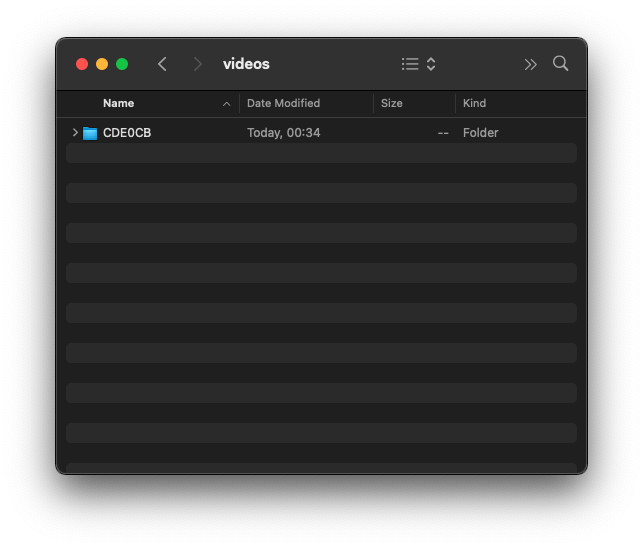
\includegraphics[width=0.7\linewidth]{../images/hls1.png}
        \caption{Папка со всеми видео}
        \label{fig:hls1}
    \end{figure}

    Внутри папки (Рис.~\ref{fig:hls2}) находятся вложенные папки, содержащие обработанные версии видео с разными разрешениями (Рис.~\ref{fig:hls3}), а также файл с расширением \emph{.m3u8}.

    \begin{figure}[h]
        \begin{center}
            \begin{minipage}[h]{0.49\linewidth}
                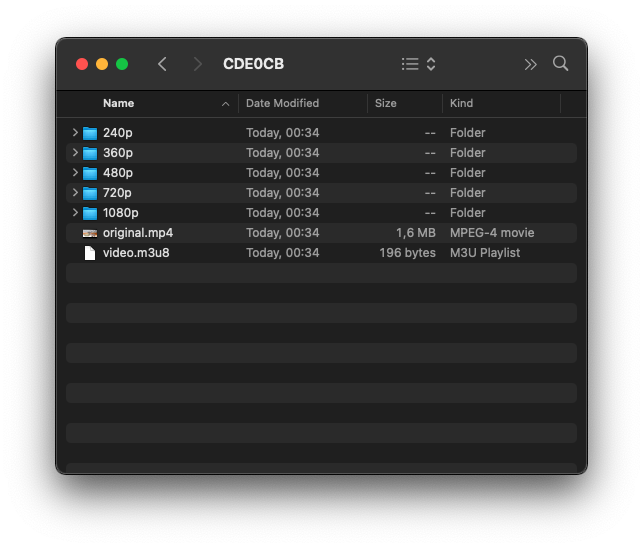
\includegraphics[width=1\linewidth]{../images/hls2.png}
                \caption{Папка видео} %% подпись к рисунку
                \label{fig:hls2} %% метка рисунка для ссылки на него
            \end{minipage}
            \hfill
            \begin{minipage}[h]{0.49\linewidth}
                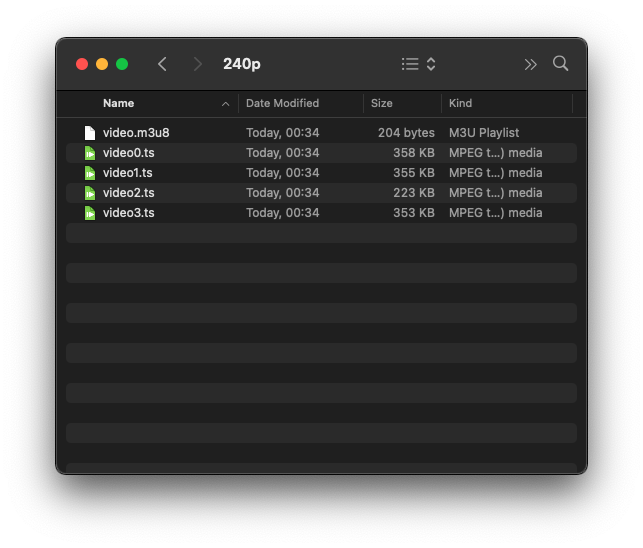
\includegraphics[width=1\linewidth]{../images/hls3.png}
                \caption{Папка отдельного разрешения}
                \label{fig:hls3}
            \end{minipage}
        \end{center}
    \end{figure}

    \subsubsection{Подключение к комнате}

    При подключении к комнате отправляем команду <<join>> на сервер.
    Сервер в ответ присылает информацию о новом клиенте и массив всех подключённых к комнате клиентов.

    \begin{lstlisting}[language=text,caption={Запрос и ответ при входе в комнату}]
    >>> SEND
    destination:/app/room/C4EC0B/join
    content-length:2

    {}


    <<< MESSAGE
    destination:/topic/room/C4EC0B/joins
    content-type:application/json
    subscription:sub-3
    message-id:llh1zcof-1426
    content-length:339

    {"notificationType":"JOIN","newUserId":"10146210-a233-4e2a-a913-691ddaaaff63","allUserIds":["10146210-a233-4e2a-a913-691ddaaaff63"],"dateTime":{"dayOfWeek":"FRIDAY","dayOfYear":134,"nano":830282000,"year":2021,"monthValue":5,"dayOfMonth":14,"hour":0,"minute":3,"second":58,"month":"MAY","chronology":{"id":"ISO","calendarType":"iso8601"}}}
    \end{lstlisting}

    \subsubsection{Отправка сообщения в чат}

    При корректной отправке команды <<chatMessage>> сервер возвращает полную информацию о полученном сообщении всем клиентам.
    Клиенты могут использовать эту информацию для отображения новых сообщений на экране пользователя.

    \begin{lstlisting}[language=text,caption={Запрос и ответ при отправке сообщения в чат}]
    >>> SEND
    destination:/app/room/C4EC0B/chatMessage
    content-length:23

    {"text":"Hello World!"}


    <<< MESSAGE
    destination:/topic/room/C4EC0B/chatMessages
    content-type:application/json
    subscription:sub-2
    message-id:eq3frfl1-1416
    content-length:316

    {"notificationType":"CHAT_MESSAGE","userId":"8c93f5fc-b8f2-4596-a681-38c4e48e8414","text":"Hello World!","dateTime":{"dayOfWeek":"THURSDAY","dayOfYear":133,"nano":981977000,"year":2021,"monthValue":5,"dayOfMonth":13,"hour":22,"minute":46,"second":55,"month":"MAY","chronology":{"id":"ISO","calendarType":"iso8601"}}}
    \end{lstlisting}

    \subsubsection{Отправка <<реакции>>}

    При корректной отправке команды <<reaction>> сервер возвращает полную информацию о полученной реакции всем клиентам.
    Клиенты могут использовать эту информацию для отображения новых реакций на экране пользователя.

    \begin{lstlisting}[language=text,caption={Запрос и ответ при отправке <<реакции>>}]
    >>> SEND
    destination:/app/room/C4EC0B/reaction
    content-length:19

    {"reaction":"GOOD"}


    <<< MESSAGE
    destination:/topic/room/C4EC0B/reactions
    content-type:application/json
    subscription:sub-1
    message-id:eq3frfl1-1417
    content-length:306

    {"notificationType":"REACTION","author":"8c93f5fc-b8f2-4596-a681-38c4e48e8414","type":"GOOD","actionTime":{"dayOfWeek":"THURSDAY","dayOfYear":133,"nano":522168000,"year":2021,"monthValue":5,"dayOfMonth":13,"hour":23,"minute":31,"second":50,"month":"MAY","chronology":{"id":"ISO","calendarType":"iso8601"}}}
    \end{lstlisting}

    \subsubsection{Отправка действий для синхронизации (воспроизведение/пауза)}

    При корректной отправке команды <<videoAction>> сервер возвращает полную информацию о полученном действии всем клиентам.
    Клиенты могут использовать эту информацию для отображения новых реакций на экране пользователя.

    У данной команды есть специальный параметр <<step>>, который может принимать значения <<CHECK>> и <<READY>>.
    При отправке действий <<воспроизведение>> и <<пауза>> сервер отправил тип <<READY>> -- это корректное поведение, дополнительно синхронизировать <<воспроизведение>> и <<паузу>> не требуется.

    \begin{lstlisting}[language=text,caption={Запрос и ответ при отправке действия для синхронизации}]
    >>> SEND
    destination:/app/room/C4EC0B/videoAction
    content-length:37

    {"seekTime":8.339047,"type":"RESUME"}


    <<< MESSAGE
    destination:/topic/room/C4EC0B/videoActions
    content-type:application/json
    subscription:sub-0
    message-id:eq3frfl1-1423
    content-length:360

    {"notificationType":"VIDEO_ACTION","actionId":-1,"author":"8c93f5fc-b8f2-4596-a681-38c4e48e8414","seekTime":8.339047,"type":"RESUME","step":"READY","actionTime":{"dayOfWeek":"THURSDAY","dayOfYear":133,"nano":23081000,"year":2021,"monthValue":5,"dayOfMonth":13,"hour":23,"minute":37,"second":34,"month":"MAY","chronology":{"id":"ISO","calendarType":"iso8601"}}}
    \end{lstlisting}

    \subsubsection{Отправка действий для синхронизации (перемотка)}

    При корректной отправке команды <<videoAction>> сервер передаёт в параметре <<step>> значение <<CHECK>> и просит подтвердить готовность к воспроизведению видео.

    \begin{lstlisting}[language=text,caption={Запрос и ответ при отправке действия для синхронизации}]
    >>> SEND
    destination:/app/room/C4EC0B/videoAction
    content-length:45

    {"seekTime":28.010935929221002,"type":"SEEK"}


    <<< MESSAGE
    destination:/topic/room/C4EC0B/videoActions
    content-type:application/json
    subscription:sub-0
    message-id:eq3frfl1-1424
    content-length:368

    {"notificationType":"VIDEO_ACTION","actionId":18,"author":"8c93f5fc-b8f2-4596-a681-38c4e48e8414","seekTime":28.010935929221002,"type":"SEEK","step":"CHECK","actionTime":{"dayOfWeek":"THURSDAY","dayOfYear":133,"nano":665335000,"year":2021,"monthValue":5,"dayOfMonth":13,"hour":23,"minute":45,"second":4,"month":"MAY","chronology":{"id":"ISO","calendarType":"iso8601"}}}
    \end{lstlisting}

    Теперь отправим команду <<videoActionReady>>, передав уникальный идентификатор действия, которое требуется подтвердить.
    В ответ сервер отправляет параметр <<step>> со значением <<READY>>.
    Таким образом, сервер ждёт готовности всех клиентов и только после этого отправляет команду на запуск.
    Поведение корректное.

    \begin{lstlisting}[language=text,caption={Подтверждение готовности воспроизвести видео}]
    >>> SEND
    destination:/app/room/C4EC0B/videoActionReady
    content-length:15

    {"actionId":18}


    <<< MESSAGE
    destination:/topic/room/C4EC0B/videoActions
    content-type:application/json
    subscription:sub-0
    message-id:eq3frfl1-1425
    content-length:367

    {"notificationType":"VIDEO_ACTION","actionId":18,"author":"8c93f5fc-b8f2-4596-a681-38c4e48e8414","seekTime":28.010935929221002,"type":"SEEK","step":"READY","actionTime":{"dayOfWeek":"THURSDAY","dayOfYear":133,"nano":34170000,"year":2021,"monthValue":5,"dayOfMonth":13,"hour":23,"minute":45,"second":5,"month":"MAY","chronology":{"id":"ISO","calendarType":"iso8601"}}}
    \end{lstlisting}

    \registrationList
\end{document}
